\documentclass[12pt,a4paper,openright,titlepage,twoside]{book}
\usepackage[T1]{fontenc} % codifica dei font
\usepackage[utf8]{inputenc} % lettere accentate da tastiera
% Includere pagine pdf (frontespizio)
\usepackage{pdfpages}
% tesi in italiano
\usepackage[italian]{babel}
% Margini: 3 cm sopra, sotto e sui lati 
\usepackage{geometry}
\geometry{a4paper,top=3cm,bottom=3cm,left=3cm,right=3cm,heightrounded}
% Interlinea 1.5
\usepackage{setspace}
\onehalfspacing
\raggedbottom
\usepackage{newtxtext,newtxmath}
% Numerazione pagine in basso a dx e sx e intestazione in alto
\usepackage{fancyhdr}
\pagestyle{fancy}
\renewcommand{\chaptermark}[1]{\markboth{\MakeUppercase{#1}}{}} %rimuovi l'enumerazione dei capitoli dall'intestazione
\renewcommand{\headrulewidth}{0.5pt}
\renewcommand{\footrulewidth}{0pt}
\fancyhf{}
\fancyfoot[LE,RO]{\thepage}
\fancyhead[LE,RO]{\slshape \rightmark}
\fancyhead[LO,RE]{\slshape \leftmark}
%headheight
\setlength{\headheight}{14.49998pt}
% Pagine bianche senza intestazione
\makeatletter
\def\cleardoublepage{\clearpage\if@twoside \ifodd\c@page\else
	\hbox{}
	\vspace*{\fill}
	\vspace{\fill}
	\thispagestyle{empty}
	\newpage
	\if@twocolumn\hbox{}\newpage\fi\fi\fi}
\makeatother
% sommario
\newenvironment{abstract}%
{\cleardoublepage%
	\thispagestyle{empty}% non rendo visibile la numerazione
	\null \vfill\begin{center}%
		\bfseries \abstractname \end{center}}%
{\vfill\null}
\providecommand{\abstract}{}
% Titoli
\usepackage{titlesec}
\titleformat{\chapter}[display]
{\normalfont\bfseries}{}{0pt}{\Huge}
\titlespacing*{\chapter}{0pt}{-50pt}{40pt}

% Bibliografia
\usepackage[autostyle, italian=guillemets]{csquotes}
\usepackage[backend=biber, style=numeric]{biblatex}
\usepackage{guit} 
\addbibresource{bibliografia.bib}
% Riferimenti incrociati
\usepackage[italian]{varioref}
% citazioni
\usepackage{quoting}
\quotingsetup{font=small}
%commenti
\usepackage{comment}
% Acronimi
\usepackage[printonlyused,withpage]{acronym}
% Figure
\usepackage{graphicx}
\usepackage[nottoc]{tocbibind}
\usepackage{wrapfig}
% svg
\usepackage{svg}
% Didascalie
\usepackage[font=small,format=hang,labelfont={sf,bf}]{caption}
\usepackage{subcaption}
% tabelle
\usepackage{tabularx}
% Codice
%\usepackage{listings}
\usepackage{listings,xcolor}
\addto\captionsitalian{%
	\renewcommand{\lstlistingname}{Codice}
	\renewcommand{\lstlistlistingname}{Elenco dei codici}}
\definecolor{codeCommentGray}{rgb}{0.55,0.55,0.55}
\definecolor{codeNaturalColorSystem}{rgb}{0,0.48,0.65}
\definecolor{codeDarkMagenta}{rgb}{0.53,0.06,0.58}
\definecolor{codeMediumDarkblue}{rgb}{0,0.20,0.70}
\definecolor{codeOliveGreen}{rgb}{0.50,0.50,0}
\definecolor{codeNumberColor}{rgb}{0.09,0.31,0.92}
\definecolor{codeDarkGreen}{rgb}{0.02,0.49,0.09}
%\definecolor{backcolour}{rgb}{0.95,0.95,0.92}
\lstdefinestyle{mystyle}{
	%	backgroundcolor=\color{backcolour},   
	commentstyle=\color{codeCommentGray},
	keywordstyle=\color{codeMediumDarkblue},
	numberstyle=\tiny, %\color{codegray},
	stringstyle=\color{codeDarkGreen},
	basicstyle=\ttfamily\footnotesize,
	breakatwhitespace=false,         
	breaklines=true,                 
	captionpos=b,                    
	keepspaces=true,                 
	numbers=left,                    
	numbersep=5pt,                  
	showspaces=false,                
	showstringspaces=false,
	showtabs=false,                  
	tabsize=2,
	frame=lines
}
%\lstset{emph={acronym,shortName,extendedName,code,correction},
	%	emphstyle=\color{codeDarkMagenta},
	%	emph={[2]Acronimo},
	%	emphstyle={[2]\color{codeNaturalColorSystem}}}
\lstset{style=mystyle}
\lstset{language=[AspectJ]Java}
\lstset{moredelim=[is][\color{codeNaturalColorSystem}]{|*}{*|}}
\lstset{moredelim=[is][\color{codeNumberColor}]{?*}{*?}}
\lstset{moredelim=[is][\color{black}]{!*}{*!}}
% Collegamenti ipertestuali e al Web
\usepackage[colorlinks]{hyperref} % sempre per ultimo
\hypersetup{
	colorlinks=true,
	linkcolor=black,
	filecolor=magenta,      
	urlcolor=cyan,
}
%\hypersetup{hidelinks}


\begin{document}
	
	\frontmatter	
	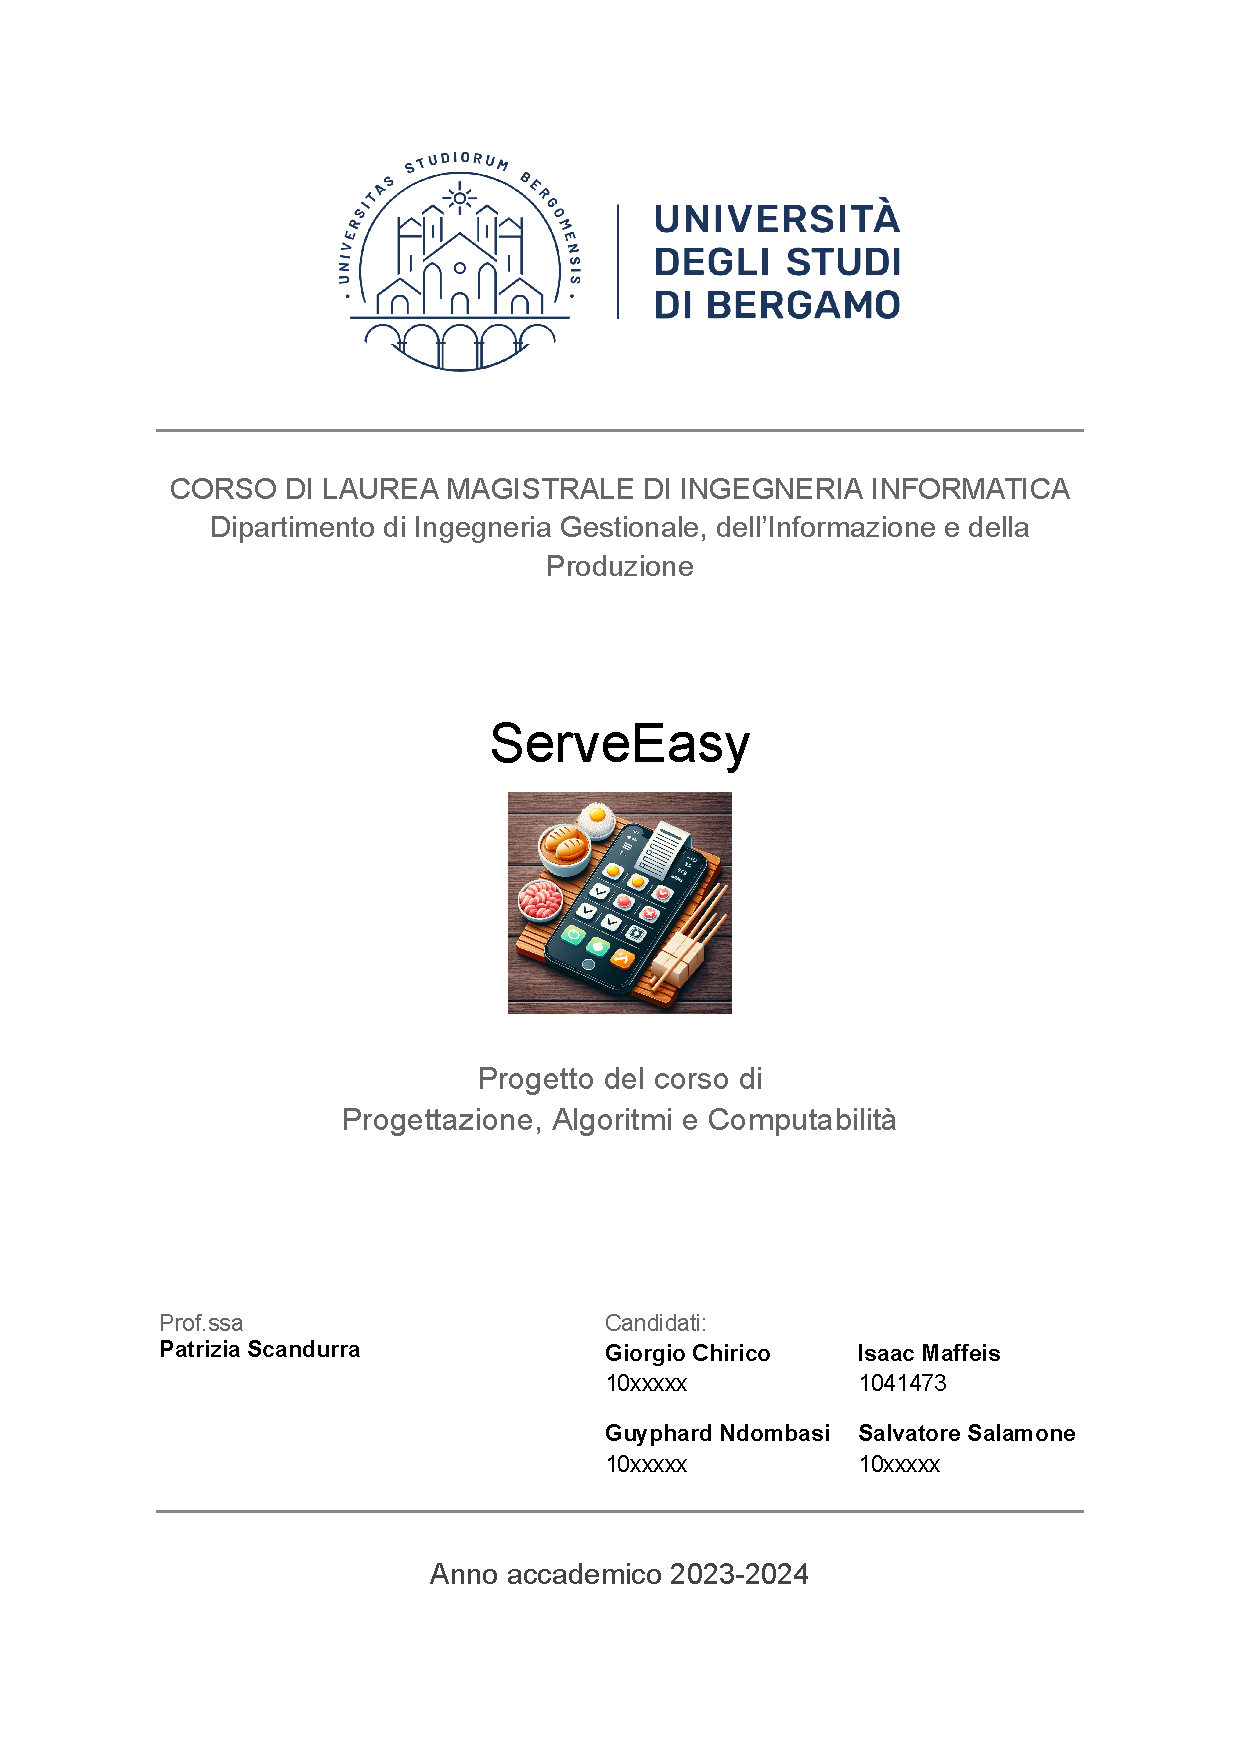
\includepdf[pages={1,{}},pagecommand={\thispagestyle{empty}}]{resources/Frontespizio.pdf}
%	\input{inizio/sommario}
	\mainmatter				
	\tableofcontents	% indice generale
	\listoffigures		% indice delle figure
	%	\lstlistoflistings  %indice del codice
	%	\addcontentsline{toc}{chapter}{Elenco dei codici}
	\chapter{Iterazione 0}
	\section{Introduzione}
Il sistema che si intende realizzare per il caso di studio è un software gestionale per ottimizzare la gestione delle comande di un ristorante, migliorando l’esperienza dei clienti, la produttività della cucina e l’efficacia della cassa.
Il sistema si baserà sull’utilizzo di tablet, che permettono ai commensali di ordinare i piatti desiderati, inserendo eventuali note, visualizzando lo stato degli ordini e richiedere il conto in modo semplice e veloce.
La cucina riceve le comande tramite una dashboard dedicata, che le ordina secondo un algoritmo di priorità basato su diversi parametri, come il tempo trascorso dall'ordinazione, la volontà del cliente, la durata di preparazione del piatto e altri fattori. La cucina può anche notificare il completamento di un ordine, che verrà visualizzato sul tablet del tavolo corrispondente. 
L’operatore di cassa sarà in grado di visualizzare il sommario degli ordini e stampare a schermo una ricevuta al cliente.
L'amministratore del ristorante può personalizzare la configurazione delle sale e dei menu, registrare i tavoli e gli account, e visualizzare delle statistiche sulle ordinazioni effettuate. Il sistema offre anche delle funzionalità opzionali, come la possibilità di far arrivare i piatti tutti insieme al tavolo, di allegare note agli ordini in preparazione, chiedere il conto al tavolo.
Il sistema si propone quindi di rendere più agile e soddisfacente il servizio di ristorazione, sfruttando le potenzialità della tecnologia e gli alti rendimenti di un algoritmo apposito.
\clearpage
	\section{Requisiti funzionali}
I requisiti funzionali sono stati esplicitati mediante il diagramma UML dei casi d’uso in \figurename~\ref{fig:use_cases_diagram}, il quale è composto da 4 attori (Amministratore, Cucina, Cassiere e Cliente che tramite ereditarietà viene ridefinito in Cliente al tavolo oppure Cliente che effettua ordinazioni d’asporto) e 6 viste (vista amministratore, vista cucina, vista cassiere, vista cliente, vista cliente al tavolo e sistema).

\begin{figure}[htbp]
	\begin{comment}
	The [htbp] option in LaTeX is used to fine-tune the placement of tables and figures.
	Each letter in [htbp] stands for a particular placement option:
	h (here): Place the table or figure in the text where the environment (like figure or table) is written, if there is enough room left on the page.
	t (top): Place it at the top of a page.
	b (bottom): Place it at the bottom of a page.
	p (page): Place it on a page containing only floats, such as figures and tables	
	LaTeX will try to place the float at the location that comes first in the option list.
	If it can’t place it there due to constraints like page size, it will move on to the next option. If none of the specified options work, LaTeX will hold the float until it finds a place where it fits, or until a \clearpage command is encountered
	\end{comment}
	\centering
	
	% verticale
	%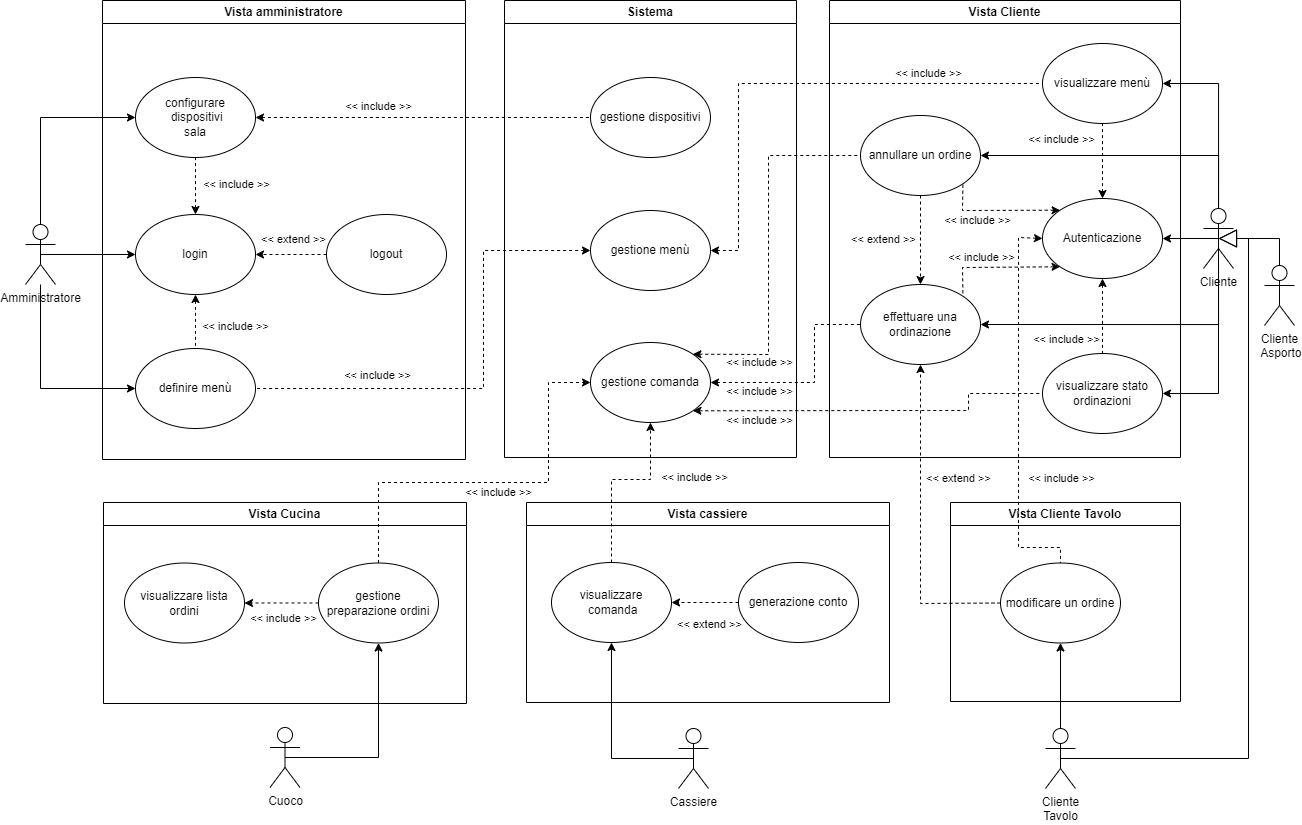
\includegraphics[scale=0.4, angle=90]{iterazione0/images/use_cases_diagram}
	
	% orizzontale
	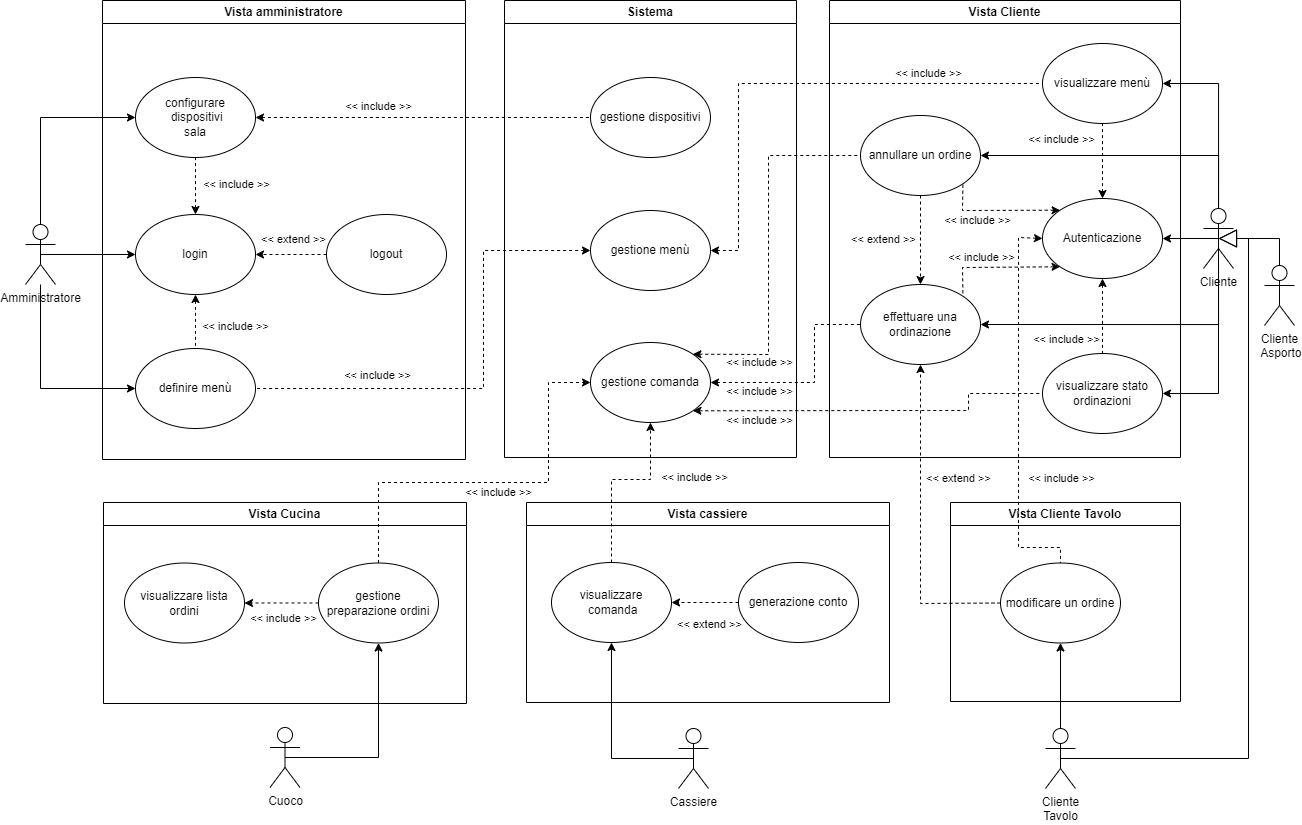
\includegraphics[scale=0.25]{iterazione0/images/use_cases_diagram}
	\caption{Diagramma dei casi d'uso\label{fig:use_cases_diagram}}
\end{figure}


Per ottimizzare il processo di sviluppo, si è deciso di categorizzare le specifiche funzionali in tabelle con tre livelli di priorità: elevata, media e bassa. Nello specifico il primo livello è assegnato alla Tabella~\ref{tab:use_cases_high_priority} a cui sono attribuiti i casi d'uso essenziali per il funzionamento dell'applicazione, i casi d'uso relativi alle funzionalità aggiuntive non critiche sono stati attribuiti alla Tabella~\ref{tab:use_cases_medium_priority} a priorità media, mentre il livello a bassa priorità che accoglie requisiti funzionali opzionali previsti per versioni successive alla Tabella~\ref{tab:use_cases_low_priority} .

\clearpage
\subsection{Priorità elevata}

\begin{table}[htbp]
	\centering
	 \begin{tabularx}{\textwidth}{|>{\centering\arraybackslash} m{4em}| >{\raggedright\arraybackslash}X |}
		\hline
		\textbf{Codice} & \textbf{Titolo} \\ [0.5ex]
		\hline\hline
		UC1 & Registrazione amministratore  \\
		\hline
		UC2 & Configurazione e gestione dispositivi (tavoli, cucina, cassa) \\
		\hline
		UC3 & Login/logout amministratore \\
		\hline
		UC4 & Gestione menù \\
		\hline
		UC5 & Algoritmo gestione coda ordini \\
		\hline
		UC6 & Cucina visualizza ordini da preparare \\
		\hline
		UC7 & Cucina notifica preparazione piatto \\
		\hline
		UC8 & Identificazione cliente \\
		\hline
		UC9 & Cliente visualizza menu \\
		\hline
		UC10 & Cliente effettua ordinazione \\
		\hline
		UC11 & Gestione sessione cliente \\
		\hline
		UC12 & Cassiere visualizza il conto \\
		\hline
	\end{tabularx}
	\caption{Casi d'uso ad elevata priorità}
	\label{tab:use_cases_high_priority}
\end{table}

\subsection{Priorità media}
\begin{table}[htbp]
	\centering
	\begin{tabularx}{\textwidth}{|>{\centering\arraybackslash} m{4em}| >{\raggedright\arraybackslash}X |}
		\hline
		\textbf{Codice} & \textbf{Titolo} \\ [0.5ex]
		\hline\hline
		UC13 & Modifica ordine al tavolo  \\
		\hline
		UC14 & Annullare un ordine \\
		\hline
		UC15 & Modifica priorità piatto (aumentare, diminuire) \\
		\hline
		UC16 & Cliente visualizza stato delle ordinazioni  \\
		\hline
	\end{tabularx}
	\caption{Casi d'uso a media priorità}
	\label{tab:use_cases_medium_priority}
\end{table}

\subsection{Priorità bassa}
\begin{table}[htbp]
	\centering
	\begin{tabularx}{\textwidth}{|>{\centering\arraybackslash} m{4em}| >{\raggedright\arraybackslash}X |}
		\hline
		\textbf{Codice} & \textbf{Titolo} \\ [0.5ex]
		\hline\hline
		UC17 & Identificazione cliente asporto  \\
		\hline
		UC18 & Cliente effettua ordinazione asporto  \\
		\hline
		UC19 & Gestione prioritaria ordinazioni da asporto \\
		\hline
		UC20 & Strategia greedy “a gruppi” (ingrediente principale in comune)   \\
		\hline
	\end{tabularx}
	\caption{Casi d'uso a bassa priorità}
	\label{tab:use_cases_low_priority}
\end{table}

\clearpage
	\section{Requisiti non funzionali}
Il progetto verrà sviluppato tenendo considerazione delle performance, integrabilità, modificabilità, testabilità e sicurezza dei componenti.

\subsection{Performance}
L'algoritmo di priorità impiegato dalla cucina per la selezione degli ordini deve fornire risultati in un tempo utile. Allo stesso tempo, gli utenti dell'applicativo web devono poter accedere e aggiornare le informazioni in un tempo accettabile.

\subsection{Integrabilità}
Ogni componente di sistema deve collaborare con gli altri componenti in modo da garantire le funzionalità previste dal sistema. Questa caratteristica è essenziale per garantire il corretto funzionamento e la coerenza dell'intero sistema.

\subsection{Modificabilità}
Il software deve facilitare l’aggiunta di nuovi componenti e funzionalità.

\subsection{Testabilità}
Ogni componente deve poter permettere la progettazione, implementazione ed esecuzione di test efficaci, in modo da garantire una massima copertura di requisiti e funzionalità.

\subsection{Sicurezza}
Il sistema deve integrare meccanismi di autenticazione ed autorizzazione degli attori, in modo da garantire la gestione delle identità, oltre alla protezione dei dati e delle API da accessi non autorizzati. Risulta dunque necessaria una distinzione dei ruoli con cui gli attori accedono al sistema.

\clearpage
	\section{Topologia}
Per il progetto è stata adottata una topologia three-tier al fine di separare in tre livelli distinti la presentazione dei dati, la gestione dell’applicativo e la mappatura dei dati sui dispositivi di archiviazione. Come si può vedere dalla \figurename~\ref{fig:topologia} il servizio è esposto tramite un web server, al quale i dispositivi clienti accedono, tramite richiesta HTTP/REST, per mezzo di una API unificata, con funzionalità di gateway. Il web-server usufruirà di database relazionali per lo storage (Data Layer), mentre sarà supportato da un database in-memory H2 (Application Layer) per avvantaggiarsi di una ridondanza dati, allo scopo di aumentare le performance lato client.

\begin{figure}[htbp]
	\centering
	
	% orizzontale
	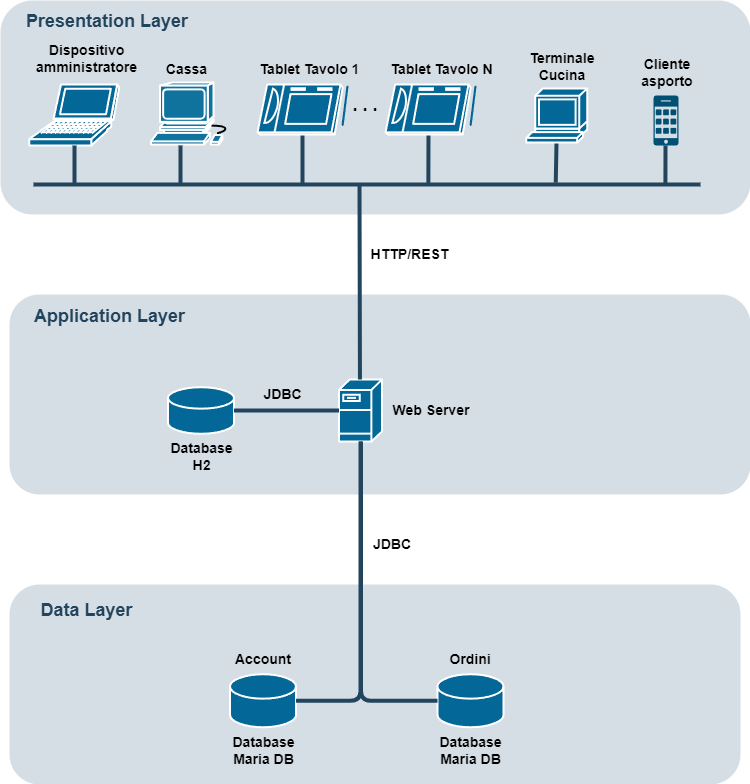
\includegraphics[scale=0.5]{iterazione0/images/topologia}
	\caption{Topologia del sistema\label{fig:topologia}}
\end{figure}

\clearpage
	\section{Toolchain}
Di seguito è presentata la toolchain utilizzata per lo sviluppo del progetto software
\subsection{Modellazione}
\begin{itemize}
	\item draw.io: casi d’uso e topologia;
\end{itemize}

\subsection{Stack applicativo}
\begin{itemize}
	\item Angular.js: front-end;
	\item Java Spring Boot 3.x.x: back-end;
	\item MariaDB: database per l’archiviazione;
	\item H2: database in-memory per rendere più efficiente l’estrazione dei dati;
\end{itemize}

\subsection{Deployment}
\begin{itemize}
	\item Docker: piattaforma per container virtuali;
	\item Docker Compose: gestione app multi-container;
\end{itemize}

\subsection{Gestore repository}
\begin{itemize}
	\item Git: Controllo versione per codice sorgente;
	\item GitHub: Piattaforma hosting e collaborativa per progetti Git;
\end{itemize}

\subsection{Continuous Integration}
\begin{itemize}
	\item Maven: gestore di progetti e dipendenze Java;
	\item GitHub Action: piattaforma di automazione per repository GitHub;
	\item Jenkins: strumento di automazione per sviluppatori;
\end{itemize}

\subsection{Analisi statica}
\begin{itemize}
	\item CodeMR su JetBrains: visualizzazione di alto livello di metriche qualitative del codice;
\end{itemize}

\subsection{Analisi dinamica}
\begin{itemize}
	\item Postman: strumento per testare API e servizi;
	\item Garfana: analisi delle performance della rete di microservizi;
	\item JUNIT: framework per test unitari Java;
\end{itemize}

\subsection{Documentazione e organizzazione del team}
\begin{itemize}
	\item Google Drive: servizio cloud per archiviazione;
	\item Documenti condivisi di Google: per elaborare la documentazione in modo condiviso;
	\item \LaTeX: generazione documentazione;
	\item Microsoft Teams: per organizzazione e meeting;
\end{itemize}

\subsection{Modello di sviluppo}
Il modello adottato segue la filosofia AGILE, con enfasi sui seguenti aspetti-chiave:
\begin{itemize}
	\item pair programming, per favorire creatività e controllo del lavoro prodotto;
	\item orientamento al risultato, con enfasi maggiore sulla generazione di codice funzionante e componenti completi prima della relativa documentazione;
	\item rapidità di risposta ai cambiamenti;
	\item collaborazione attiva col cliente, al fine di incontrare le sue necessità, garantire trasparenza e fornire feedback tempestivo sul lavoro di progetto;
	\item Proattività nell’identificazione e mitigazione dei rischi.
\end{itemize}

\clearpage
	\chapter{Iterazione 1}
	\section{Introduzione}
Il sistema che si intende realizzare per il caso di studio è un software gestionale per ottimizzare la gestione delle comande di un ristorante, migliorando l’esperienza dei clienti, la produttività della cucina e l’efficacia della cassa.
Il sistema si baserà sull’utilizzo di tablet, che permettono ai commensali di ordinare i piatti desiderati, inserendo eventuali note, visualizzando lo stato degli ordini e richiedere il conto in modo semplice e veloce.
La cucina riceve le comande tramite una dashboard dedicata, che le ordina secondo un algoritmo di priorità basato su diversi parametri, come il tempo trascorso dall'ordinazione, la volontà del cliente, la durata di preparazione del piatto e altri fattori. La cucina può anche notificare il completamento di un ordine, che verrà visualizzato sul tablet del tavolo corrispondente. 
L’operatore di cassa sarà in grado di visualizzare il sommario degli ordini e stampare a schermo una ricevuta al cliente.
L'amministratore del ristorante può personalizzare la configurazione delle sale e dei menu, registrare i tavoli e gli account, e visualizzare delle statistiche sulle ordinazioni effettuate. Il sistema offre anche delle funzionalità opzionali, come la possibilità di far arrivare i piatti tutti insieme al tavolo, di allegare note agli ordini in preparazione, chiedere il conto al tavolo.
Il sistema si propone quindi di rendere più agile e soddisfacente il servizio di ristorazione, sfruttando le potenzialità della tecnologia e gli alti rendimenti di un algoritmo apposito.
\clearpage
	\section{Component Diagram}
\subsection{Sistema ServeEasy}
\subsubsection{single component del sistema}
\begin{figure}[H]
	\centering
	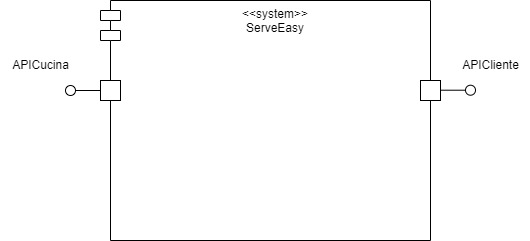
\includegraphics[scale=0.6]{iterazione1/images/ServeEasy_componente_unico.jpg}
	\caption{Component diagram - ServeEasy\label{fig:component_diagram_serveeasy}}
\end{figure}
Visualizzazione iniziale della soluzione come un componente unico che espone due API, dedicate rispettivamente alla cucina ed ai clienti. Si procede con uno sviluppo top-down.

\subsubsection{primo zoom-in sul sistema}

\begin{figure}[H]
	\centering
	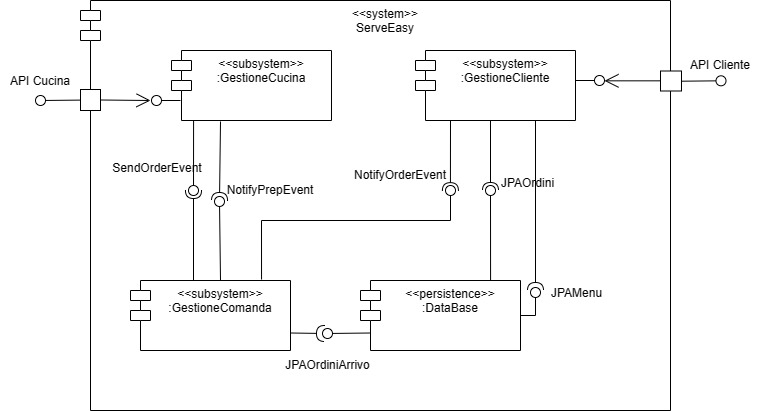
\includegraphics[scale=0.5]{iterazione1/images/ServeEasy_primo_zoomin.jpg}
	\caption{Component diagram - System\label{fig:component_diagram_system}}
\end{figure}
Al primo zoom-in si identificano i servizi che andranno a comporre l’architettura della soluzione:
\begin{itemize}
	\item \textbf{GestioneComanda:} risolve gli use case del gruppo “sistema”, rappresenta il cuore del sistema ed incorpora la logica di backend fondamentale per la gestione regolarizzata degli ordini da cliente a cucina, attraverso politiche di schedulazione a priorità progettate ed implementate con un algoritmo ad-hoc.
	\item \textbf{GestioneCliente:} risolve gli use case del gruppo “cliente”, espone le funzionalità destinate ai dispositivi di tavolo ed al portale web per clienti d’asporto. Ha dunque il compito di gestire gli aspetti del servizio legati alle interazioni del cliente col sistema, come la visualizzazione del menu, la creazione degli ordini ed il raggruppamento degli ordini in una comanda relativa.
	\item \textbf{GestioneCucina:} risolve gli use case del gruppo “cucina”, espone le chiamate destinate ai dispositivi di cucina. Questo servizio conterrà un sistema a code, dove l’ordine in arrivo verrà classificato ed inserito in base al suo ingrediente principale. Gli ordini verranno gestiti dalle postazioni della cucina seguendo una politica FIFO.
\end{itemize}
Per la memorizzazione persistente dei dati cruciali per l’attività come piatti, ordini e comande, è stato inserito un componente database.
All’interno del sistema ServeEasy, i componenti comunicano tra loro attraverso una comunicazione ad eventi, asincrona. Si è deciso di attuare una politica pub-sub per la gestione delle comunicazioni interne, costituite da scambi di notifiche e DTO tra i microservizi designati.

\subsection{Gestione Comanda}
\subsubsection{Componenti esagonali}
Il design dei microservizi seguirà l’architettura esagonale: un dominio, denominato “Domain”, nucleo della logica di servizio, sarà racchiuso tra due gusci denominati “Interface” e “Infrastructure”, i quali avranno il compito di astrarre la gestione dati, rendendola opaca al dominio. La logica di base del microservizio seguirà lo schema port-adapter, dove il dominio comunica con i gusci attraverso delle interfacce dette porte (il cui nome nel progetto è caratterizzato dal suffisso “Port”), mentre i gusci hanno il compito di implementare l’effettivo componente di trasmissione (guscio Infrastructure) e/o ricezione (guscio Interface), detto adattatore (sarà identificabile da suffisso “Adapter”). 
Nello specifico il \textbf{Domain} definisce gli oggetti, le entità e le operazioni che sono pertinenti al problema che il microservizio gestisce.Gli \textbf{Interface adapters} fungono da ponte tra il mondo esterno e il core del sistema, consentendo al microservizio di comunicare con altre applicazioni, servizi o dispositivi esterni in modo indipendente dall'implementazione interna del sistema stesso, mentre gli \textbf{Infrastructure adapters} fungono da ponte tra il core del sistema e l'infrastruttura esterna, gestendo le chiamate e le operazioni necessarie per accedere e utilizzare le risorse infrastrutturali.
Tali caratteristiche avvantaggiano l’intercambiabilità dei singoli componenti di sistema a costo di un aumento della complessità.
\begin{figure}[H]
	\centering
	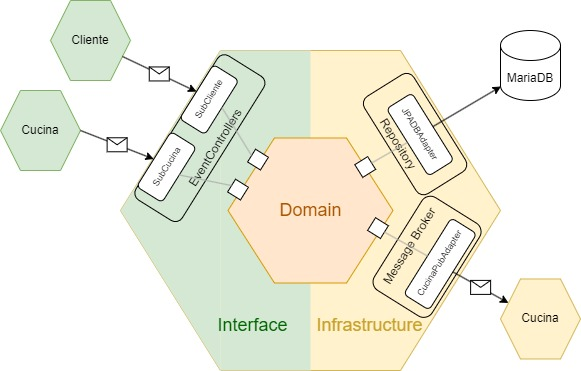
\includegraphics[scale=0.7]{iterazione1/images/hexagon.jpg}
	\caption{Architettura esagonale per il microservizio Gestione comanda\label{fig:hexagon}}
\end{figure}

\subsubsection{zoom-in gestione comanda}
\begin{figure}[H]
	\centering
	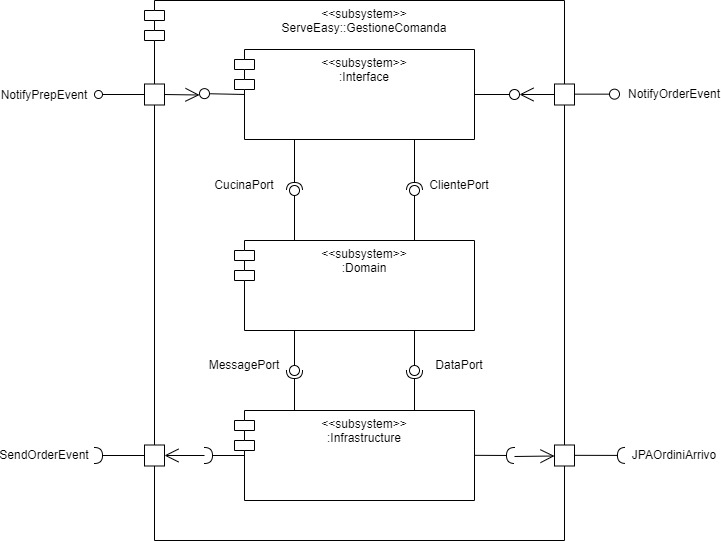
\includegraphics[scale=0.5]{iterazione1/images/component_comanda_cucina-GestioneComanda.jpg}
	\caption{Component diagram - Gestione Comanda\label{fig:component_diagram_gestione_comanda}}
\end{figure}


\subsubsection{zoom-in infrastructure di gestione comanda}
\begin{figure}[H]
	\centering
	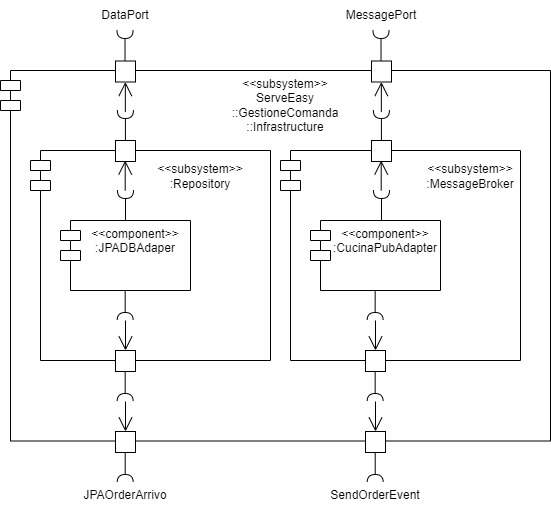
\includegraphics[scale=0.5]{iterazione1/images/component_comanda_cucina-GestioneComanda__Infrastructure.jpg}
	\caption{Component diagram - Gestione Comanda - Infrasrtructure \label{fig:component_diagram_gestione_comanda_infrastracture}}
\end{figure}

\subsubsection{zoom-in domain di gestione comanda}
\begin{figure}[H]
	\centering
	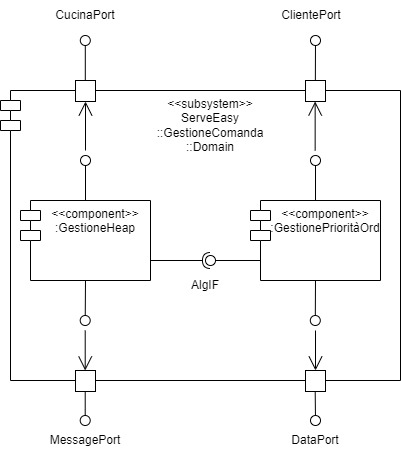
\includegraphics[scale=0.5]{iterazione1/images/component_comanda_cucina-GestioneComanda__Domain.jpg}
	\caption{Component diagram - Gestione Comanda - Domain \label{fig:component_diagram_gestione_comanda_domain}}
\end{figure}

\subsubsection{zoom-in interface di gestione comanda}
\begin{figure}[H]
	\centering
	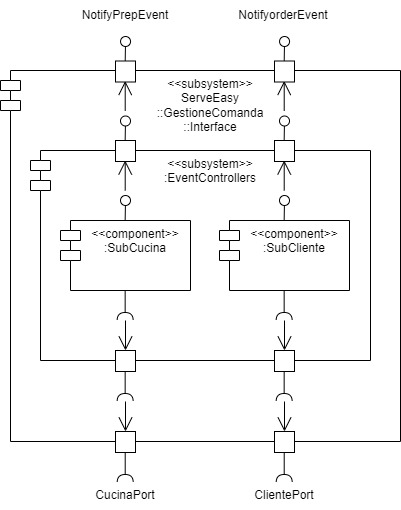
\includegraphics[scale=0.5]{iterazione1/images/component_comanda_cucina-GestioneComanda__Interface.jpg}
	\caption{Component diagram - Gestione Comanda - Interface \label{fig:component_diagram_gestione_comanda_interface}}
\end{figure}

\subsection{Gestione Cucina}
\subsubsection{zoom-in gestione cucina}
\begin{figure}[H]
	\centering
	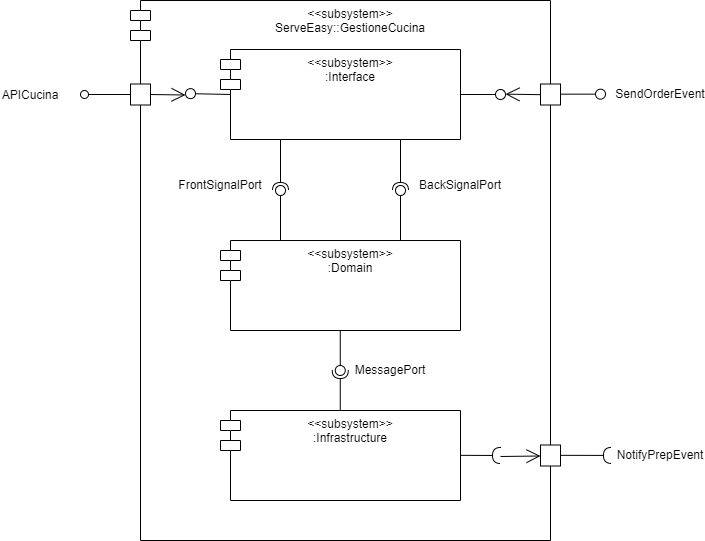
\includegraphics[scale=0.5]{iterazione1/images/component_comanda_cucina-GestioneCucina.jpg}
	\caption{Component diagram - Gestione Cucina \label{fig:component_diagram_gestione_cucina}}
\end{figure}

\subsubsection{zoom-in infrastructure di gestione cucina}
\begin{figure}[H]
	\centering
	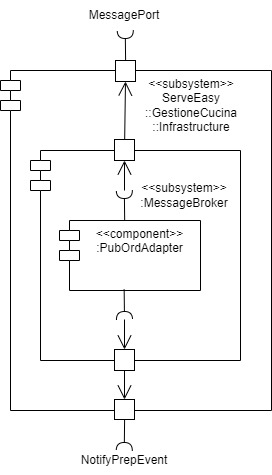
\includegraphics[scale=0.5]{iterazione1/images/component_comanda_cucina-GestioneCucina__Infrastructure.jpg}
	\caption{Component diagram - Gestione Cucina - Infrastructure \label{fig:component_diagram_gestione_cucina_infrastructure}}
\end{figure}

\subsubsection{zoom-in domain di gestione cucina}
\begin{figure}[H]
	\centering
	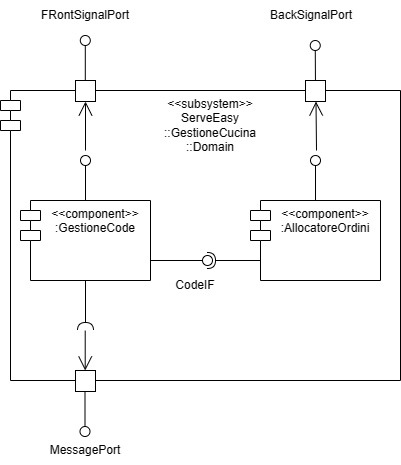
\includegraphics[scale=0.5]{iterazione1/images/component_comanda_cucina-GestioneCucina__Domain.jpg}
	\caption{Component diagram - Gestione Cucina - Domain \label{fig:component_diagram_gestione_cucina_domain}}
\end{figure}

\subsubsection{zoom-in interface di gestione cucina}
\begin{figure}[H]
	\centering
	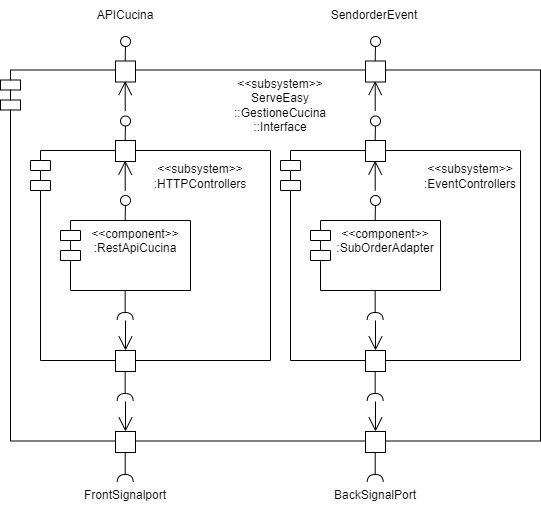
\includegraphics[scale=0.5]{iterazione1/images/component_comanda_cucina-GestioneCucina__Interface.jpg}
	\caption{Component diagram - Gestione Cucina - Interface \label{fig:component_diagram_gestione_cucina_interface}}
\end{figure}

\subsection{Gestione Cliente}
\subsubsection{zoom-in gestione cliente}
\begin{figure}[H]
	\centering
	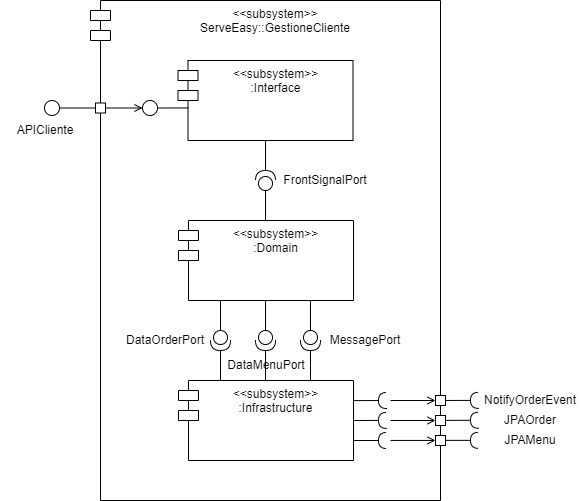
\includegraphics[scale=0.5]{iterazione1/images/GestioneCliente_subsystem-GestioneCliente.jpg}
	\caption{Component diagram - Gestione Cliente \label{fig:component_diagram_gestione_cliente}}
\end{figure}

\subsubsection{zoom-in infrastructure di gestione cliente}
\begin{figure}[H]
	\centering
	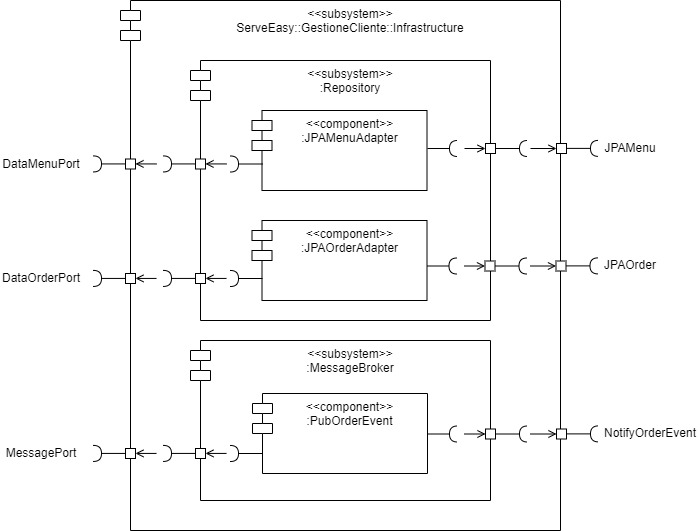
\includegraphics[scale=0.5]{iterazione1/images/GestioneCliente_subsystem-Infrastructure.jpg}
	\caption{Component diagram - Gestione Cliente - Infrastructure \label{fig:component_diagram_gestione_cliente_infrastructure}}
\end{figure}

\subsubsection{zoom-in domain di gestione cliente}
\begin{figure}[H]
	\centering
	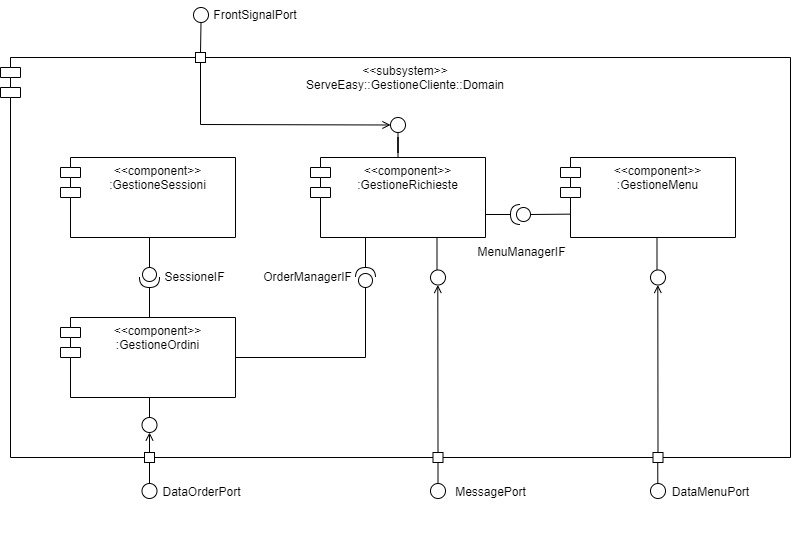
\includegraphics[scale=0.5]{iterazione1/images/GestioneCliente_subsystem-Domain.jpg}
	\caption{Component diagram - Gestione Cliente - Domain \label{fig:component_diagram_gestione_cliente_domain}}
\end{figure}

\subsubsection{zoom-in interface di gestione cliente}
\begin{figure}[H]
	\centering
	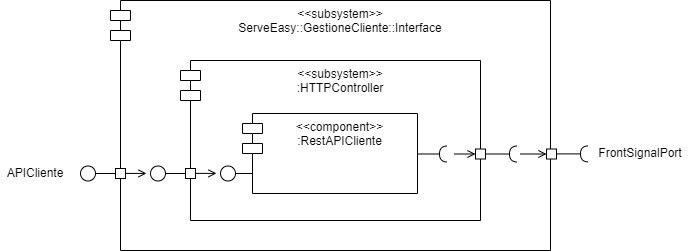
\includegraphics[scale=0.5]{iterazione1/images/GestioneCliente_subsystem-Interface.jpg}
	\caption{Component diagram - Gestione Cliente - Interface \label{fig:component_diagram_gestione_cliente_interface}}
\end{figure}

\clearpage
	\backmatter	
	%	\input{fine/acronimi}
%	\input{fine/bibliografia}
	
\end{document}